\section{Устойчивые и неустойчивые задачи. Жесткие системы.}

\subsection*{Устойчивые и неустойчивые задачи}

Рассматривается поведение решений следующих задач
\[\begin{array}{ccc}
    y'_1=y      & y'_2=-y_2      & y'_3=-2(x-1)y_3    \\
    y_1(x)=ce^x & y_2(x)=ce^{-x} & y'_3=ce^{-(x-1)^2}
  \end{array}\]

Интегральные кривые первого семейства расходятся с увеличением $x$,
второго  сближаются, а третьего  сначала расходятся, а затем сближаются.
Так как на $k$-ом шаге найденное приближенное значение $y_k$ смещается с
интегральной кривой $y_{k-1}(x)$, то внесенная в результате этого
погрешность может в зависимости от поведения семейства решений
либо возрастать, либо уменьшаться, см. рис.:

\begin{figure}[h]
  \begin{minipage}{.3\linewidth}
    \centering
    \tikzsetnextfilename{16/IncreasingExp}
    \begin{tikzpicture}
      \draw [domain=0:2.6] plot function{0.10*exp(x)};
      \draw [domain=0:2.6] plot function{0.15*exp(x)};
      \draw [domain=0:2.6] plot function{0.20*exp(x)};
    \end{tikzpicture}
    \caption*{$Ce^x$}
  \end{minipage}\hfill
  \begin{minipage}{.3\linewidth}
    \centering
    \tikzsetnextfilename{16/DecreasingExp}
    \begin{tikzpicture}
      \draw [domain=0:3] plot function{1*exp(-x)};
      \draw [domain=0:3] plot function{2*exp(-x)};
      \draw [domain=0:3] plot function{3*exp(-x)};
    \end{tikzpicture}
    \caption*{$Ce^{-x}$}
  \end{minipage}\hfill
  \begin{minipage}{.3\linewidth}
    \centering
    \tikzsetnextfilename{16/IncDecExp}
    \begin{tikzpicture}
      \draw [domain=0:3] plot function{1*exp(-(x-1)**2)};
      \draw [domain=0:3] plot function{2*exp(-(x-1)**2)};
      \draw [domain=0:3] plot function{3*exp(-(x-1)**2)};
    \end{tikzpicture}
    \caption*{$Ce^{-(x-1)^2}$}
  \end{minipage}
\end{figure}

В связи с этим имеется существенная разница в численном интегрировании
двух на первый взгляд эквивалентных задач

\[\begin{array}{cc} \begin{cases}y'_1=y_1 \\ y_1(0)=1\end{cases} & \begin{cases}y'_2=e^x \\ y_2(0)=1\end{cases} \end{array}\]

так как соответствующие им семейства интегральных кривых существенно
отличаются: $y(x) = ce^x$, $y(x) = c+e^x$.

Выясним, какое из рассмотренных уравнение явный метод
Эйлера проинтегрирует точнее. Пусть при внесении начальных
данных внесется погрешность $\delta_0>0$, то есть $y_0=y(0)+\delta_0$

\begin{enumerate}
  \item Посчитаем глобальную погрешность для первой задачи:
        \[\frac{y_{k+1}-y_k}{h}=y_k\Rightarrow y_{n}=(1+h)y_{n-1}=(1+h)^{1/h}y_0=(1+h)^{1/h}(y(0)+\delta_0)=(1+h)^{1/h}(1+\delta_0)\]
        \[(1+h)^{\frac{1}{h}}=\exp\left\{\frac{1}{h}\ln(1+h)\right\}=\exp\left\{1-\frac{h}{2}+\bigO(h^2)\right\}=e\cdot\left(1-\frac{h}{2}+\bigO(h^2)\right)\]
        \[\abs{y(x_n)-y_n}=\abs{e-e\cdot\left(1-\frac{h}{2}+\bigO(h^2)\right)(1+\delta_0)}= e\frac{h}{2}+e\delta_0\left(1+\frac{h}{2}\right)+\bigO(h^2)\]
  \item Посчитаем глобальную погрешность для второй задачи:
        \[\frac{y_{k+1}-y_k}{h}=e^{x_k}\Rightarrow y_{n}=y_{n-1}+he^{x_{n-1}}=\sum_{i=0}^{n-1}he^{x_i}+\delta_0\]
        Полученная расчетная формула соответстует составной формуле прямоугольника
        по крайней точке. Для такой формулы позднее будет получена
        оценка
        \[\abs{y(x_n)-\sum_{i=0}^{n-1}he^{x_i}-\delta_0}\leq\abs{y(x_n)-\sum_{i=0}^{n-1}he^{x_i}}+\delta_0\leq \norm{(e^x)'}_{x\in[0,1]}\frac{(1-0)^2}{2N}+\delta_0=e\frac{h}{2}+\delta_0\]
\end{enumerate}

Вывод: вторая схема проинтегрирует точнее. Стоит обратить внимание,
что погрешность вносится не только при задании $y_0$, но
и при каждом вычислении. В случае первой задачи такая погрешность будет
расти экспоненциально, в отличие от второй задачи.

\subsection*{Жесткие схемы}

Рассмотрим задачу интегрирования уравнения $y'=-ay,\ a\equiv\const>0,\ x\in[0,X]$.
Для решения данной задачи запишем явную разностную схему
\[\frac{y_{k+1}-y_k}{h}=-ay_{k}\Rightarrow y_{k+1}=(1-ha)y_k\]

Решение исходной дифференциальной задачи убывает при увеличении $x$.
Логично требовать, чтобы решение разностной задачи
тоже обладало этим же качеством: $\abs{1-ha}<1$.
Соответствующее множество шагов $h$ называется \textit{областью устойчивости}
разностной схемы, а максимально допустимый шаг $h_{cou}=2/a$ - \textit{числом Куранта}.

Так как $y(x+h)=y(x)+hy'(x)+\frac{h^2}{2}y''(\xi),\ x\leq\xi\leq x+h$,
то погрешность аппроксимации имеет вид $\abs{\frac{h^2}{2}y''(\xi)}$.
Величина $y''(\xi) = a^2e^{-a\xi} \ll 1$ при $a\xi\gg1$. Поэтому при
$a\xi\gg1$ для достижения требуемой точности локальной аппроксимации
$\abs{hy''(\xi)}\leq\varepsilon$ не требуются мелкие шаги, но $h \leq h_{cou}$
для всех $x$ из условия качественного совпадения решений (условия устойчивости).

Данный пример показывает, что разумно выделить класс так называемых \textit{жестких
  задач}. Будем считать задачу $y'=f$ жесткой, если \textit{характерное время изменения
  решения много меньше отрезка интегрирования} (в данном случае это означает,
что $aX \gg 1$). Система уравнений $y = Ay, y = (y_1,\ldots,y_n)^T$ считается жесткой,
если

\[
  1)\ \text{Re}(\lambda_i(A))>0 \quad
  2)\ s=\frac{\max_i\abs{\text{Re}(\lambda_i(A))}}{\min_i\abs{\text{Re}(\lambda_i(A))}} \gg 1
\]

Число $s$ принято называть \textit{числом жесткости}. Данное определение обобщается на случай матриц $A(x)$.

В случае одного уравнения задача будет жесткой, если решение содержит
несколько компонент с существенно отличающимися характерными
временами изменения. Рассмотрим задачу
\[y' = -a(y-\sin x)+\cos x,\ y(0) = 1,\ a \gg 1\Rightarrow y(x) = e^{-ax} + \sin x\]
Здесь можно выделить пограничный слой быстрого изменения решения, далее решение
мало отличается от плавной функции $\sin x$. Однако $\forall\ x$ необходимо выполнение условия $h \leq h_{cou}$.

\begin{figure}[h]\label{fig:courant_with_explicit_schemes}
  \begin{minipage}{.3\linewidth}
    \centering
    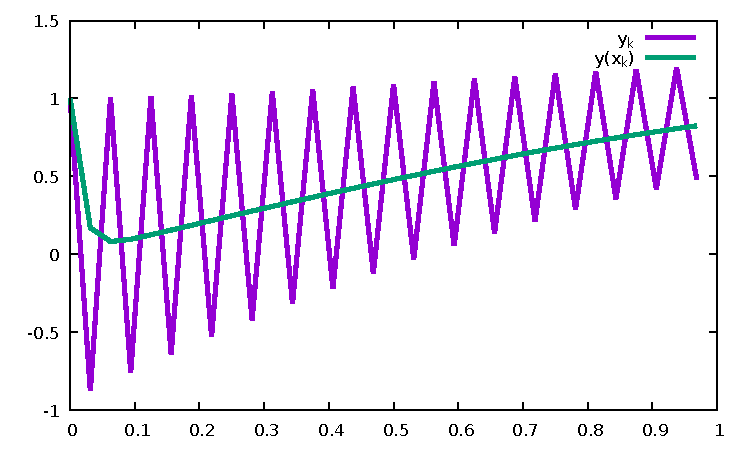
\includegraphics[scale=0.4]{16/ConvergingCosineScheme.pdf}
    \caption*{$N=32$, $X=1$, $A=63$}
  \end{minipage}\hfill
  \begin{minipage}{.3\linewidth}
    \centering
    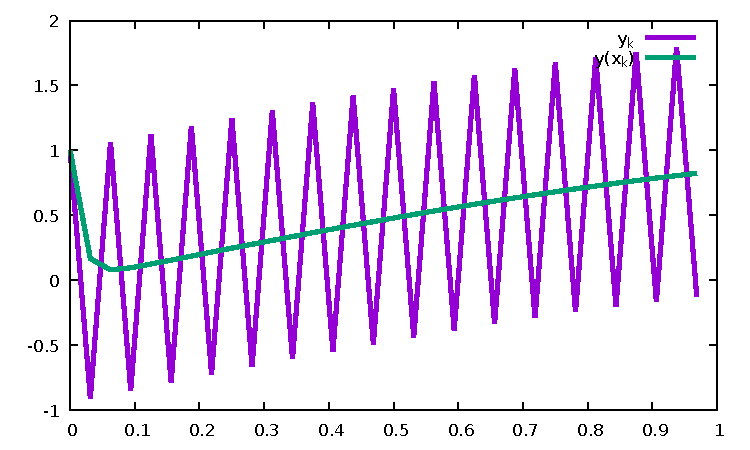
\includegraphics[scale=0.4]{16/StableCosineScheme.pdf}
    \caption*{$N=32$, $X=1$, $A=64$}
  \end{minipage}\hfill
  \begin{minipage}{.3\linewidth}
    \centering
    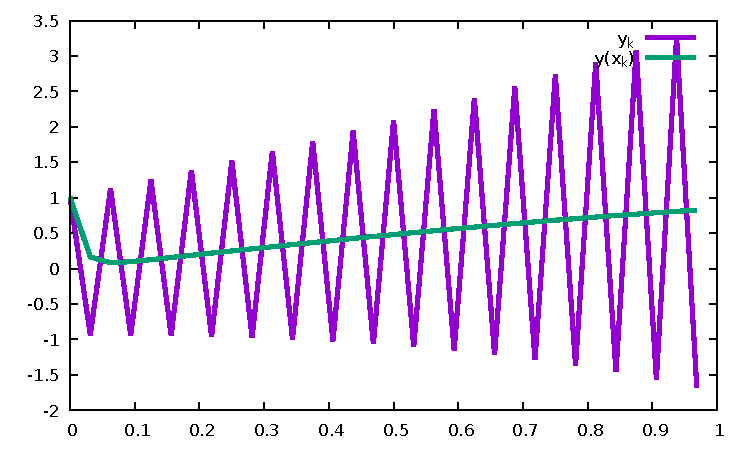
\includegraphics[scale=0.4]{16/UnstableCosineScheme.pdf}
    \caption*{$N=32$, $X=1$, $A=65$}
  \end{minipage}
  \caption{Результаты явной схемы Эйлера с различными входными параметрами}
\end{figure}

Еще раз отметим, что устойчивость дифференциальной задачи определяется
типом уравнения и значениями параметров, устойчивость разностной задачи -
типом разностной схемы, значениями параметров и величиной шага.
Так явные схемы с постоянным шагом обычно требуют мелких шагов, но просты в реализации.
Неявные схемы обычно имеют менее жесткие условия на $h$ за счет дополнительных вычислений в общем случае.

\begin{figure}[h]
  \centering
  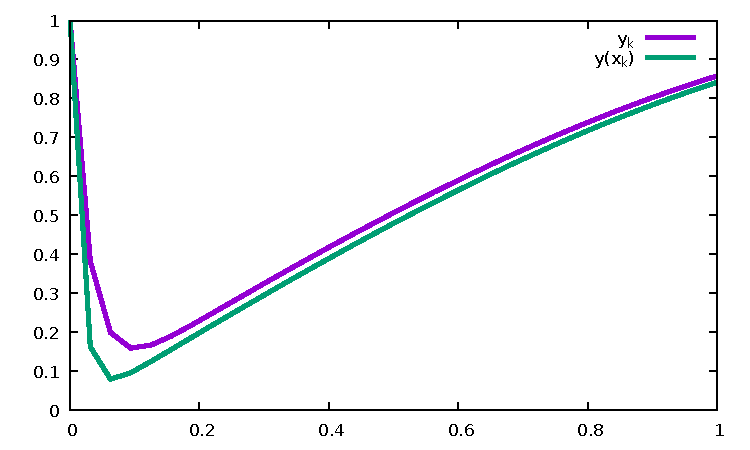
\includegraphics[scale=0.4]{16/ImplicitCosineScheme.pdf}
  \caption{Результаты неявной схемы Эйлера с $N=32$, $X=1$, $A=65$}
\end{figure}
